\documentclass[12pt]{report}
\usepackage[a4paper,left=30mm,right=25mm,top=25mm,bottom=25mm]{geometry}
\usepackage[utf8]{inputenc}
\usepackage[english,hungarian]{babel}
\usepackage{t1enc}
\usepackage{graphicx}
\usepackage{caption}
\usepackage{marginnote}
\usepackage{listings}
\usepackage{color}
\usepackage{newtxtext,newtxmath} % times new roman imitation
\usepackage{graphicx}
\usepackage{setspace}
\usepackage{tabularx}
\usepackage{mathtools}
\usepackage{float}
\usepackage{fancyhdr}
\usepackage{makeidx} % indexing enable
\graphicspath{ {images/} }
\usepackage{emptypage}

\newcommand\blankpage{%
    \null
    \thispagestyle{empty}%
    \addtocounter{page}{-1}%
    \newpage}

\usepackage[totoc]{idxlayout}

\linespread{1.5}

\makeindex

% Equation capture settings
\DeclareCaptionType{equ}[][List of equations]
\captionsetup[equ]{labelformat=empty}

% Figure caption settings
\renewcommand{\thefigure}{\arabic{chapter}-\arabic{figure}}

% Table caption settings
\renewcommand{\thetable}{\arabic{chapter}-\arabic{table}}

% Code listing styles
\definecolor{codegreen}{rgb}{0,0.6,0}
\definecolor{codegray}{rgb}{0.5,0.5,0.5}
\definecolor{codepurple}{rgb}{0.58,0,0.82}
\definecolor{backcolour}{rgb}{0.95,0.95,0.92}

\lstdefinestyle{codestyle}{
    backgroundcolor=\color{backcolour},   
    commentstyle=\color{codegreen},
    keywordstyle=\color{magenta},
    numberstyle=\tiny\color{codegray},
    stringstyle=\color{codepurple},
    basicstyle=\ttfamily\footnotesize,
    breakatwhitespace=false,         
    breaklines=true,                 
    captionpos=b,                    
    keepspaces=true,                 
    numbers=left,                    
    numbersep=5pt,                  
    showspaces=false,                
    showstringspaces=false,
    showtabs=false,
    escapeinside={\%(*}{*)},
    tabsize=2
}
\lstset{style=codestyle}

\usepackage[bibstyle=authoryear,
            citestyle=authoryear,
            backend=biber,
            sorting=nyt]{biblatex}
\addbibresource{bibliography.bib}

\usepackage{hyperref}

\renewcommand{\labelenumii}{\roman{enumii})} % list: second level is roman numerals

\title{
TERMÉSZET ÁLTAL INSPIRÁLT OPTIMALIZÁCIÓS MEGOLDÁSOK
}

\author{Kiss Gergely}
\date{Temesvár, 2022}

\begin{document}

\makeatletter
\renewcommand\maketitle{
{
\begin{center}

\includegraphics{logo} \\[4ex]
\Large \uppercase{Tudományos diákköri dolgozat}
\end{center}
%\raggedright % Note the extra {
\vspace{1cm}
\begin{center}
{\Huge \bfseries \uppercase{\@title} }\\
\vspace{2cm}
\newcolumntype{R}{>{\raggedleft\arraybackslash}X}%
\centering
\large{
\begin{tabularx}{\textwidth}{R X}
\textbf{Szerző:} &  \textbf{\@author} \\
         & Számítástechnika MSc. szak, I. évf. \\[4ex]
\textbf{Konzulens:} & \textbf{dr. Lendák Imre} \\
& egyetemi tanár
\end{tabularx}
}
\end{center}}
} % Note the extra }

\begin{titlepage}
\thispagestyle{fancy}
\fancyhf{}
\renewcommand{\headrulewidth}{0pt}
\cfoot{Temesvár, 2022}
\maketitle
\end{titlepage}

\blankpage
\newpage
\pagenumbering{gobble}
\linespread{1}

\begin{center}
    {\bfseries
    \vspace*{1.5cm}
    \large{SAPIENTIA ERDÉLYI MAGYAR TUDOMÁNYEGYETEM} \\\vspace{2.5cm}
    \large{\@title} \\ \vspace{1.5cm}
    \large{NATURE INSPIRED OPTIMIZATION SOLUTIONS} \\ \vspace{2cm}
    }
    \large{
    \@author \\ \vspace{2cm}
    
    Konzulens: \\
    dr. Lendák Imre
    \vfill
    Kézirat lezárva: 2022. március 26.
    }
\end{center}

\blankpage
\blankpage
\selectlanguage{english}
\begin{abstract}
    
The aim of this study is to present optimization algorithms which were inspired by nature and to analyze their accuracy. Accuracy plays an important role in optimization solutions, so the main goal of these algorithms is to ensure efficient and relatively accurate results. The study presents the genetic algorithm and the particle-swarm algorithm as two prominent members of the evolutionary algorithms.

One of the main advantages of evolutionary algorithms is that they can optimize any criterion function even if it’s mathematically impossible to get a result. The evolutionary algorithms’ common features are their parameters: population number and the number of iterations. They influence the accuracy and the speed of the algorithm aswell. Areas of application of these algorithms include machine learning, artificial neural networks, big data analysis.

I used various tools to perform the analysis: for the genetic algorithm I used \textit{Matlab}’s \textit{Optimization Toolbox} package, on the other hand I used my own \textit{Python} and \textit{Javascript} program to evaluate the particle swarm optimization algorithm. I chose the Rastrigin function as the criterion function. Each experiment was performed 100x which ultimately calculated mean, median and standard deviation. I got comparable results after a few sets of these experiments where every set of calculations were carried out with different parameters. These analyzes have shown that these algorithms do not always give accurate results and it is always the best to make compromises in terms of speed and accuracy depending on the optimization problem.

Keywords: optimization, evolutionary algorithms, genetic algorithm, particle swarm optimization.

\end{abstract}
\blankpage
\selectlanguage{hungarian}
\begin{abstract}

A dolgozat célja bemutatni olyan optimalizációs algoritmusokat, melyek létrejöttét a természet inspirálta, valamint kivizsgálni ezen algoritmusok pontosságát. Optimalizációs megoldásoknál nagy szerepet kap a pontosság, így ezek az algoritmusoknak is fő céljuk a hatékony és relatív pontos eredmény biztosítása. A dolgozat a genetikus algoritmust valamint a részecske-raj algoritmust mutatja be, mint az evolúciós algoritmusok két jeles tagját.

Az evolúciós algoritmusok fő előnyei közé tartozik, hogy bármilyen kritériumfüggvényt optimalizálni tudnak, így a matematikai úton lehetetlen eredményt is ki tudják számolni. Közös vonásaik a paramétereikben húzódnak, miszerint a populációszámuk és a ciklusszámuk befolyásolja az algoritmusok pontosságát és gyorsaságát elsősorban. Az evolúciós algoritmusok felhasználási területe többek között a gépi tanulás, mesterséges neuronhálózatok, big data analízis.

A kísérletek lebonyolításához különböző segédeszközöket használtam: a genetikus algoritmushoz a \textit{Matlab} szoftvercsomag \textit{Optimization Toolbox} nevű modulját, míg a részecske-raj optimalizációnál saját kezűleg írt \textit{Python} illetve \textit{Javascript} szoftvert használtam. Kritériumfüggvényként a Rastrigin-féle függvényt választottam. Kísérletenként 100 számítást végeztem, ami végeredményül középértéket, mediánt és szórást számolt ki. A különböző kísérleteket különböző paraméterek mellett ismételtem meg, így összehasonlítható eredményekre jutottam. Az elemzések kimutatták, hogy ezek az algoritmusok – báris a kezdetleges változatuk – nem minden esetben szolgálnak pontos eredménnyel, így kompromisszumos megoldásokat lehet csak ajánlani az algoritmus gyorsasága és pontossága terén.

Kulcsszavak: optimalizáció, evolúciós algoritmusok, genetikus algoritmus, részecske-raj optimalizáció.

\end{abstract}
\blankpage
\selectlanguage{hungarian}
%\addtocontents{toc}{\protect\thispagestyle{empty}}
\pagenumbering{gobble}
\tableofcontents
\listoffigures
\listoftables
\blankpage\blankpage
%\listofequs
\newpage
\pagenumbering{arabic}
\setcounter{page}{1}

\chapter{Bevezető}

A modern kori mérnöki tudományokban egyre nagyobb teret hódítanak azok a megoldások, amelyek a természet jól bevállt működési elvét, strukturális felépítését imitálják. A biomimetika/bionika egy egész tudományág, ami ezekkel a természetbeli megoldások mérnöki megvalósításával foglalkozik.

A műszaki tudományokban lépten-nyomon szembetaláljuk magunkat optimalizációs problémákkal. Alapvető fizikai törvényszerűségeket is fel lehet állítani, mint optimalizációs probléma: például az energia megmaradási törvénye. Teljesen jogos tehát azt állítani, hogy a természet végzi a legtöbb optimalizációt.

Ha már a természet ilyen jól tud optimalizálni, feltétlenül léteznie kell olyan megoldásoknak, amelyek követnek valamiféle természetes folyamatokat. Ebben a dolgozatban két ilyen megoldás kerül bemutatásra, amely egyszerűen és hatékonyan oldja meg az optimalizációs problémákat: a genetikus algoritmus és a részecske-raj optimalizáció. Ezek az algoritmusok sztochasztikus folyamatok\footnote{A sztochasztikus folyamat, vagy más néven véletlenszerű folyamat, az a folyamat, melyet -- részben vagy teljesen -- valószínűségi változók jellemeznek. Ennek az ellentéte a determinisztikus folyamat, ahol a folyamatot leíró változók nem véletlenszerűek \parencite{wikipedia2020}} \index{sztochasztikus folyamat}, amelyek az evolúciós algoritmusok családjába tartoznak.

Ha a természet olyan összetett folyamatot, mint az optimalizáció képes lebonyolítani, akkor az ember csakis természetes folyamatok által tudja ezt a feladatot leghatékonyabban elvégezni. A fent említett algoritmusok bemutatása és elemzése előtt viszont érdemes megismerkedni az optimalizáció matematikai definíciójával.
\chapter{Matematikai optimalizáció}

Ebben a fejezetben a matematikai optimalizáció elméleti háttere kerül bemutatásra.

\section{Matematikai optimalizáció definíciója}

Matematikai optimalizáció \index{matematikai optimalizáció} alatt olyan folyamatot értünk, amely egy előre meghatározott kritérium alapján keresi a legjobb megoldást \parencite{vujanovic1980}. Ezt az eredményt hívjuk optimális értéknek. Az optimalizáció kritériumfüggvényét\footnote{Kritériumfüggvény. Szinonímái: költségfüggvény, energiafüggvény, hasznossági függvény.} \index{kritériumfüggvény} a \ref{eq:criteria} képlettel ábrázoljuk.

\begin{equ}[!ht]
  \begin{equation}
    \begin{aligned}
        f: &X \to Y, Y \subseteq R \\
        f &= f(x) \\
        x &= x_1, x_2, ..., x_n
    \end{aligned}
  \end{equation}
  \caption{\label{eq:criteria}}
\end{equ}

Az optimalizáció valós esetben a \ref{eq:criteria} függvény minimális vagy maximális értékének a meghatározását jelenti, vagyis minimum esetében a \ref{eq:min} képlet, maximum esetében a \ref{eq:max} képlet érvényes.

\begin{equ}[!ht]
  \begin{equation}
    f(x^*) \leq f(x), \forall x \in X
  \end{equation}
  \caption{\label{eq:min}}
\end{equ}

\begin{equ}[!ht]
  \begin{equation}
    f(x^*) \geq f(x), \forall x \in X
  \end{equation}
  \caption{\label{eq:max}}
\end{equ}

Mivel a fenti esetekben a függvény legkisebb (illetve legnagyobb) értékét az egész értelmezési tartomány szintjén az $x^*$ adja meg, ezért ezt globális optimalizációnak\footnote{Globális optimalizáció kiterjed az egész értelmezési tartomány szintjére. Lokális optimalizáció esetében csak az $x^*$ közelében vizsgáljuk a függvényt: $\parallel x^* - x \parallel < \varepsilon$} nevezzük.

A kritériumfüggvény mellett más egyenletek (\ref{eq:g} képlet) is szerepelhetnek a probléma meghatározásában.

\begin{equ}[!ht]
  \begin{equation}
    g_k(x) = 0
  \end{equation}
  \caption{\label{eq:g}}
\end{equ}

Ilyenkor korlátos vagy megkötött matematikai optimalizációról beszélünk. A továbbiakban csak megkötés nélküli optimalizációról lesz szó.

\section{Optimalizációs módszerek}

Sokféle analitikus módszer segítségével lehet eljutni a kritériumfüggvény optimális értékéhez. Többségük a függvény többszörös differenciálhatóságát követeli meg, így összetettebb esetekben ezeket a módszereket nem tudjuk alkalmazni. Ahogy nő a probléma dimenzionalitása, úgy válik nehezebbé az analitikus eredmény kiszámítása (ha egyáltalán lehetséges az analitikus eredményig eljutni). Ilyenkor az egyedüli megoldást a numerikus módszerek \index{numerikus módszer} jelentik.

Tegyük fel, hogy a számítógép segítségét kérjük ennek a problémának a megoldásában. Milyen módszerhez kell folyamodnunk, hogy a várt eredményt kapjuk meg? Legrosszabb esetben végigfutnánk az összes elemen, és így megtalálnánk a keresett legjobb értéket. Ez egyrészt nem kivitelezhető, mert a függvényeink általában folytonos térben mozognak, így végtelen számú elemet kellene leellenőrizni. Ha mégis valahogy felosztanánk a függvény dómenjét $N$ részre, az rettenetesen hosszú számítási időt venne igénybe. Egyedüli megoldást a numerikus algoritmusok kínálnak \parencite{rapaic2019}.

\chapter{Evolúciós algoritmusok}

A numerikus módszerek előnye, hogy viszonylag gyorsan, bármilyen függvény esetében tudnak eredménnyel szolgálni, nincsenek különleges követelményeik, mint az analitikus módszerek esetében.

A számítástechnikai irodalomban nagyszámú sztochasztikus optimalizációs algoritmus létezik, egyik csoportjuk ezeknek az evolúciós algoritmusok. Ezeknek az algoritmusoknak az a különlegessége, hogy véletlenszerű változókat tartalmaznak, így két egymás utáni, egyforma feltételek mellett lezajlott számítás nem fog pontosan egyforma eredményt adni.

Az evolúciós algoritmusok, mint ahogy az a nevükben is szerepel, a természetes evolúció működését próbálják imitálni. Közös vonásuk, hogy egyidőben több lehetséges eredménnyel számolnak, ezeknek a halmaza alkotja a \textit{populációt} \index{populáció}. Ez a populáció ciklusról-ciklusra változásokon megy keresztül úgy, hogy minden ciklusban egyre közelebb kerüljön az optimális értékhez.

Ebben a dolgozatban az evolúciós algoritmusok közül két képviselőjük kerül bemutatásra: a genetikus algoritmusok és a részecske-raj algoritmus.

\chapter{Genetikus algoritmus}

Az élővilág egyik alappillére a szaporodás, ami biztosítja a fajok túlélését hosszú távon. Az evolúciós törvényeket betartva azok a fajok maradnak fenn legtovább, akik jobban tudtak alkalmazkodni a környezetükhöz; a vadonban a legnagyobb, legerősebb, legtalálékonyabb fajok vannak előnyben, így szaporodáskor is nagyobb esélyük van pont ezeket a géneket továbbadni. Minél jobb génekkel rendelkezik egy élőlény, annál életrevalóbb utódjai lesznek, és ezzel növelik az egész faj esélyét a túlélésre. R. A. Fisher\footnote{Ronald Aylmer Fisher (1890--1962) brit statisztikus, genetikus} még az 1950-es években fejlesztette ki azt a matematikai modellt, amelyet a mai formába John Henry Holland\footnote{John Henry Holland (1929--2015) amerikai számítástechnika és pszichológia professzor} ültetett át, és manapság genetikus algoritmusnak \index{genetikus algoritmus} hívunk \parencite{holland2012}.

\section{A genetikus algoritmus alapjai}

A genetikus algoritmus populációját olyan egyedek (ún. kromoszómák) alkotják, amelyek géneket hordoznak magukban. A gének száma megegyezik az optimalizációs probléma dimenzionalitásával, vagyis általános esetben $n$ darab génnel rendelkezik az egyed. Minden kromoszóma a keresési mezőben potenciális megoldás lehet, így mindre ki tudjuk számolni a kritériumfüggvény értékét, ami az egyed alkalmasságát jelenti. A genetikus algoritmus célja, hogy az egyedek génjeit úgy változtatja meg, hogy azok alkalmassági értékei a lehető legjobbak legyenek, így megtalálva az optimális értéket. A kromoszómák génjeit \textit{genetikus műveletek} \index{genetikus műveletek} segítségével lehet változtatni.

\section{A genetikus műveletek}

Ebben a részben különféle genetikus műveleteket mutatunk be.

\subsection{Kiválasztás}

Általános esetben a populációt $N$ darab kromoszóma alkotja, melyeknek az alkalmassági értékein kell javítani. A genetikus elméletet követve a legjobb génekkel rendelkező egyedeknek kell utódokat létrehozniuk annak érdekében, hogy az egész populáció génállományát erősítsék. Tehát minden új ciklusban (generációban) meg kell ismételni a genetikus műveleteket. Egyszerre két egyedet kell kijelölni úgy, hogy a kiválasztás valószínűsége egyenesen arányos legyen az egyed alkalmasságával.

Egy efféle algoritmus a \textit{rulettkerék kiválasztás} \index{rulettkerék kiválasztás}, ami minden egyednek biztosít egy mezőt a keréken, de a mező szélessége egyenesen arányos az egyedhez rendelt kiválasztási valószínűséggel. Első gondolatra ez nem is tűnik rossz megoldásnak, másrészt viszont olyan mellékhatás léphet fel, ami szuper-egyedeket generál: így nem tudjuk biztosítani a globálisan elérhető optimumot, ha a szuper-egyed egy lokális optimumban akad meg. Ez a szuper-egyed később magához vonza a többi egyedet is, így a globális optimumot mind elkerüli \parencite{kanovic2017}.

Ahhoz, hogy ne favorizáljunk túl bizonyos géneket, rang alapú rendszert kell bevezetni, ahol az egyedek az alkalmassági értékük alapján vannak sorrendbe állítva, és $1$-től $N$-ig terjedő számmal vannak megjelölve. Tehát egy nagyon jó génekkel ellátott egyed és egy kevésbé jó géneket hordozó egyed között sokkal kisebb ez esetben a különbség.

\subsection{Keresztezés}

A kiválasztott egyedek képezik azt a halmazt, amiből majd kikerülnek a jövendőbeli szülők. Az utódok keresztezés útján jönnek létre, és így örökölnek bizonyos tulajdonságokat a felmenőiktől. Ez a művelet változtatja a populáció helyzetét, vagyis egyenes úton manipulálja a kromoszómák génszerkezetét.

A keresztezést többféle módon lehet kivitelezni:

\begin{itemize}
    \item binárisan kódolt gének uniform keresztezése (\ref{fig:keresztezes} ábra)
    
Két szülőtől két utód jön létre olyan módon, hogy egy véletlenszerűen generált bit-maszkot használva keverjük össze a szülők génjeit. (Az első utód az első szülőtől kap egy gént, ha a bit-maszkban 0 szerepel, ha pedig 1-es, akkor a második szülőtől. A második utód pedig ellenkező logikával kapja meg a génjeit).

\begin{figure}
    \centering
    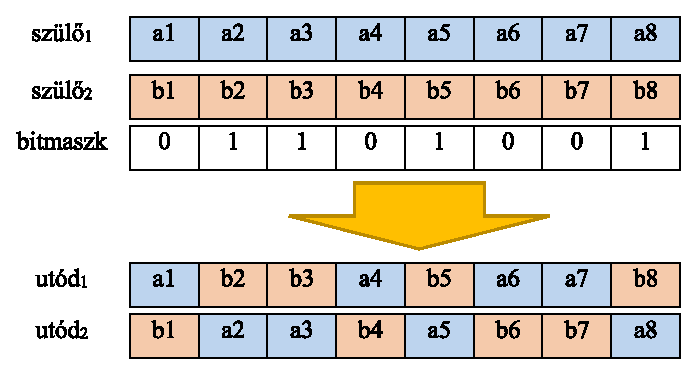
\includegraphics[width=0.75\textwidth]{keresztezes}
    \caption{Bináris uniform keresztezés \parencite{kanovic2017}}
    \label{fig:keresztezes}
\end{figure}

    \item reális számokkal kódolt gének aritmetikai keresztezése
    
A reális számoknál is hasonló keresztezés által születnek meg az utódok. A szülők ($x_1$ és $x_2$) génjeinek lineáris kombinációja alkotja az utódok génjeit (\ref{eq:keresztezes} képlet).

\begin{equ}[!ht]
  \begin{equation}
    \begin{aligned}
      x_1^0 &= a \cdot x_1 + (1-a) \cdot x_2 \\
      x_2^0 &= a \cdot x_2 + (1-a) \cdot x_1
    \end{aligned}
  \end{equation}
  \caption{\label{eq:keresztezes}}
\end{equ}

Ebben az esetben az a paraméter egy véletlenszerű szám 0 és 1 között, ami megfelel az előző példában szereplő bit-maszknak.
\end{itemize}

\subsection{Mutáció}

Mint ahogy az a természetes evolúcióban is jelentkezik, a gének időszakonként mutálódnak, így egy olyan populáció jön létre, amely nagyon kis mértékben eltér az előző generációtól. Ez azért fontos, mert ezek a kis mutációk jelentik azt a génbeli sokszínűséget, ami ellenállóbbá teszi az egyedeket (pl. kórokozók ellen).

A genetikus algoritmusban azért van szükség mutációra, hogy ne részesítsünk előnyben bizonyos egyedeket, amik így nem válnak szuper-egyedekké. Habár ezt a genetikus műveletet elenyésző számú egyeden végzik el, mégis gyorsabb konvergenciót eredményez, mintha mutáció nélkül zajlott volna az algoritmus \parencite{kanovic2017}.

Valós számok esetében a mutáció a következőképp végezhető el:

\begin{itemize}
    \item a génhez tartozó valós számot egy véletlenszerű valós számmal váltjuk fel (legdrasztikusabb hatást vált ki),
	\item nullához közeli valós szám hozzáadása vagy kivonása, vagy
	\item egyhez közeli valós számmal való szorzás.
\end{itemize}

Miután befejeztük a genetikus műveleteket, el kell dönteni, hogy mely egyedek kerülnek be a következő generációba. A legegyszerűbb módszer az újonann kapott egyedeket átmenti a következő generációba, míg az összes szülőt kitörli a keresési mezőből. Ezzel az a gond, hogy egyes rendkívül jó génekkel rendelkező szülő le lesz cserélve egy estleges kevésbé jó utódra. Az ilyen probléma kiküszöbölésére alkalmazzák az \textit{elitizmus} \index{elitizmus} elvét, miszerint bizonyos kritériumoknak megfelelő szülő át lesz mentve a következő generációra és potenciálisan lehet még utódja. Ez segíti az algoritmus konvergencióját, de elővigyázatosan kell kiválasztani azt a bizonyos elit kritériumot; különben létrejön egy \textit{szuper-egyed} \index{szuper-egyed}, ami nem minden esetben a globális optimumot mutatja \parencite{kanovic2017}.

\section{A genetikus algoritmus elemzése}

A genetikus algoritmus empírikus analíziseként a szakirodalom tesztfüggvények elemzését ajánlja \parencite{kanovic2017}. Ebben a dolgozatban bemutató jelleggel csak egy ún. Rastrigin-féle tesztfüggvény \index{Rastrigin-függvény} elemzése kerül elemzésre.

A Rastrigin-féle függvény érdekessége, hogy sok lokális minimuma van, és a \ref{eq:rastrigin} képlettel van definiálva. A függvény háromdimenziós grafikonja a \ref{fig:rastrigin3d} ábrán megtekinthető, valamint a függvény x-y síkra tett vetülete (\ref{fig:rastriginxy} ábra).

\begin{equ}[!ht]
  \begin{equation}
    f(x) = 10n + \sum_{i=1}^{n} (x_i^2 - 10 \cos(2 \pi x_i))
  \end{equation}
  \caption{\label{eq:rastrigin}}
\end{equ}

Általános esetben a függvény optimális értéke: $f(x^*)=0$, $x^*=[0,0,...,0]$, míg kétdimenziós probléma esetében ($n=2$): $f(x^*)=0$, $x^*=[0,0]$.

\begin{figure}
    \centering
    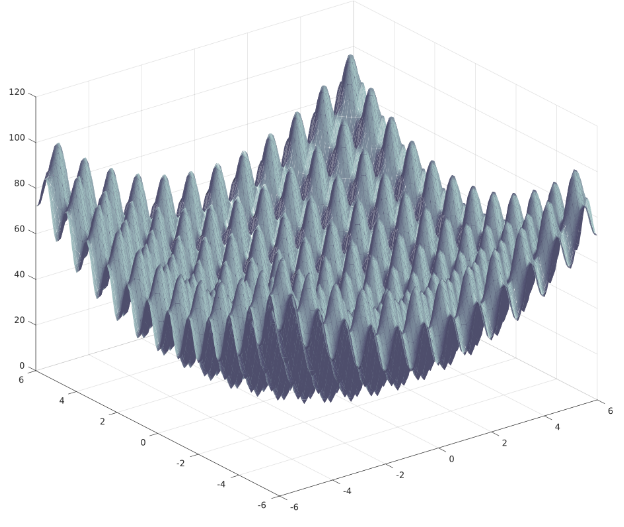
\includegraphics[width=0.8\textwidth]{rastrigin3d}
    \caption{Rastrigin-függvény grafikonja}
    \label{fig:rastrigin3d}
\end{figure}

\begin{figure}
    \centering
    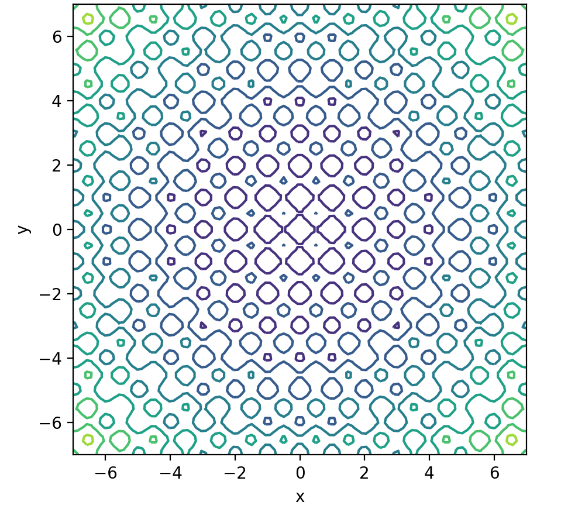
\includegraphics[width=0.8\textwidth]{rastriginxy}
    \caption{Rastrigin-függvény x-y vetülete}
    \label{fig:rastriginxy}
\end{figure}

A számításokat a \textit{Matlab} szoftvercsomag \textit{Optimization Toolbox} \parencite{matlab2016} moduljával végeztem. Négy különböző környezetben zajlott a számítás, más-más paraméterek mellett (generációszám és populációszám).

\linespread{1}
\begin{lstlisting}[language=Matlab, caption={A Rastrigin-függvény kódja}, captionpos=b]
function v = rastrigin(x)
	A = 10;
	s = sum(x.*x - A * cos(2*pi*x));
	v = A * length(x) + s;
end
\end{lstlisting}

A kísérletet százszoros megismétlése után születtek meg az eredmények, melyek a \ref{tab:genresult} táblázatban találhatók. Mindemellett az egyedek kezdőpozíciói elrendezettsége kétféle módon lett meghatározva: uniform elrendezettség (zöld), nem uniform elrendezettség (kék).

\begin{table}
    \centering
    \begin{tabular}{|m{0.5cm}|m{2.5cm}|m{2.5cm}|m{8cm}|}
    \hline
    \# & populációszám & generációszám & eredmények \\ \hline
    \hline
    K1 & 25 & 200 & 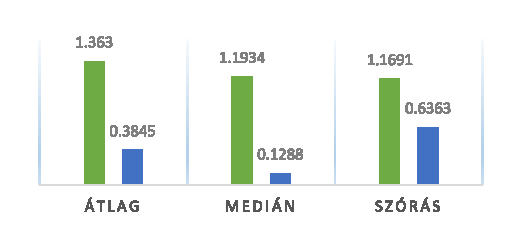
\includegraphics{gen1} \\ \hline
    K2 & 25 & 400 & 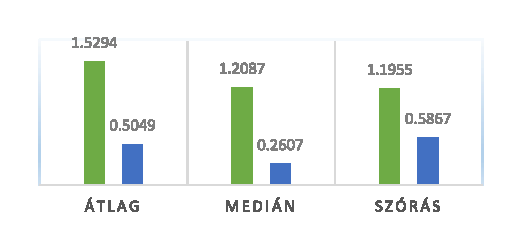
\includegraphics{gen2} \\ \hline
    K3 & 100 & 200 & 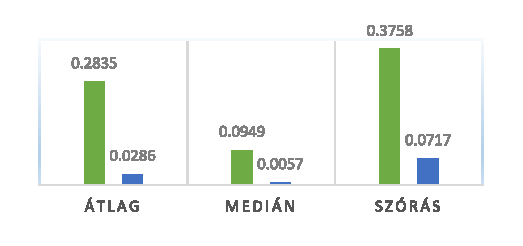
\includegraphics{gen3}	\\ \hline
    K4 & 200 & 200 & 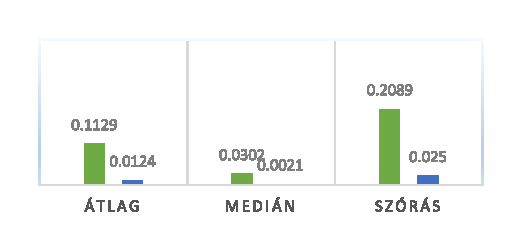
\includegraphics{gen4} \\ \hline
    \end{tabular}
    \caption{A Rastrigin-függvény elemzésének az eredményei}
    \label{tab:genresult}
\end{table}

Az eredmények alapján megállapíthatjuk, hogy a generáció számának a növelésével nem javult az eredményünk pontossága, míg a populáció számának a növelése nagyban hozzájárult a jobb eredményhez. A genetikus algoritmusnál a populáció számának a növelése drasztikusan lassítja az optimalizációs folyamatot, így a probléma sajátosságaihoz képest kell eldönteni, hogy gyors és kevésbé pontos eredményt kapunk, vagy lassú de pontosabb eredményt.

A legérdekesebb eredmények viszont az egyedek kezdőpozícióinak a változtatásakor születtek. Minden esetben jobb eredményt ért el az algoritmus, amikor a keresési mezőn nem egyenletesen (\ref{fig:uniform} ábra), hanem tömbben (\ref{fig:notuniform} ábra) helyezte el az egyedeket.

\begin{figure}
    \centering
    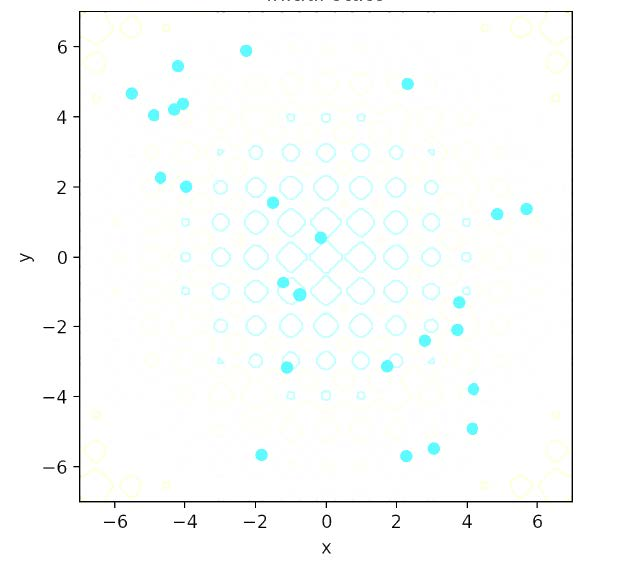
\includegraphics[width=0.7\textwidth]{uniform}
    \caption{Részecskék uniform kezdőpozíciói}
    \label{fig:uniform}
    \centering
    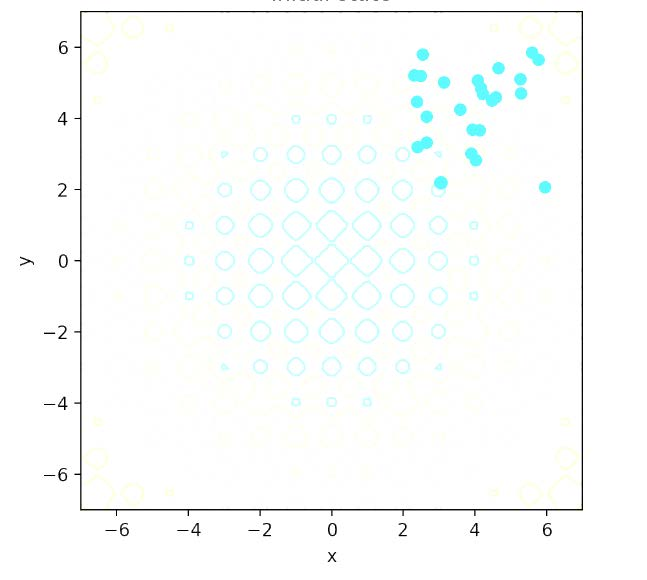
\includegraphics[width=0.7\textwidth]{notuniform}
    \caption{Részecskék nem-uniform kezdőpozíciói}
    \label{fig:notuniform}
\end{figure}

Az eredmények függvényében megállapítható, hogy a genetikai algoritmus jobban teljesít, ha kevesebb egyed nagyobb koncentrációban jelenik meg a keresési mezőn. A konkrét problémára levetítve ez jobb irányelvnek bizonyult, de más problémák esetében javasolt a paraméterek és a kezdőpozíció finomhangolása.

\section{A genetikus algoritmus felhasználási területei}

A genetikus algoritmus egy megbízható és állóképes algoritmus, mint amilyen a természetes evólúció is, amelyről modellezték. Rendkívűl széleskörű a használata: a matematikától kezdve, az egészségügyön át, a különböző mérnöki szakirányzatokig. A genetikus műveletek többféle módon való értelmezése különböző előnyöket ad a genetikus algoritmus felhasználásának más és más szakterületen: kombinatorikus problémák megoldása, képfeldolgozás, mesterséges neuronhálózatok és más gépi tanulási technikák \parencite{kanovic2017}.

\chapter{Részecske-raj optimalizáció}

Ebben a fejezetben a részecske-raj optimalizáció kerül bemutatásra.

\section{Rajintelligencia}

Az állatok alapvető túlélési ösztönei közé tartozik az élelem és élőhely utáni keresés. Ez minden állatfajra igaz, a hangyától a bálnáig, mégis a csoportokban élő állatfajok különösen egymásra vannak utalva ilyen téren. Az oka ennek, hogy külön-külön valószínűleg elpusztulnának, de csoportokban sokkal erősebbek és védettebbek lesznek. Ezt a jelenséget nevezik \textit{rajintelligenciának} \index{rajintelligencia}, miszerint a nem-intelligens egyedek intelligens viselkedésmintákat mutatnak csoportokban, ami végül sikeres túlélési képességet eredményez \parencite{rapaic2019}.

1995-ben James Kennedy amerikai pszichológus és Russel C. Eberhart mérnök pontosan definiálták ezeket a viselkedésmintákat, és így született meg a részecske-raj optimalizáció \parencite{dorigo2007}.

\section{A részecske-raj optimalizáció alapjai}

A részecske-raj optimalizációs algoritmus \index{részecske-raj algoritmus} populációja olyan egyedekből áll, amelyek állandó mozgásban tartják az egész rajt. Ez a mozgás nagyban függ az egyed saját tapasztalataitól, vagyis az eddigi bejárt úttól. Az így megszerzett információk alapján az egyedek egymással kommunikálnak, és a lehető legjobb eredmény felé mozdulnak el. Ez a mozgás ciklusonként frissül, ami a gyakorlatban annyit jelent, hogy lépésenként változik a raj helyzete. A genetikus algoritmustól eltérően a populáció tagjai nem cserélődnek, mindig ugyanazok az egyedek szerepelnek a rajban, csak a helyzetük változik.

Ha a sorrendben $n$-edik ciklus keresztmetszetét vesszük, minden részecske a következő információkat hordozza magával:

\begin{itemize}
    \item a részecske jelenlegi helyzete -- $x[n]$:
a keresési tartomány egyik értéke, dimenzionalitása függ a kritériumfüggvény dimenziójától;
	\item jelenlegi sebesség -- $v[n]$:
a részecske előző lépésből szerzett sebessége (az előző helyzettől való elmozdulása);
	\item a részecske eddigi legjobb helyzete -- $p[n]$:
a részecskének az a pozíciója, amelyet eddigi útja során felvett, és a legjobb értéket hordozza.
\end{itemize}

A fent említett paraméterek mellett fontos még a raj szintjén történő információcsere, vagyis a raj szintjén elért eddigi legjobb helyzet -- $g[n]$. Ez a paraméter a valaha elért legjobb részecske helyzetét jelenti.

A részecskék térben és időben történő változását a \ref{eq:vn} és a \ref{eq:xn} egyenletek határozzák meg.

\begin{equ}[!ht]
  \begin{equation}
    v[n+1] = w \cdot v[n] + cp \cdot rp[n] \cdot (p[n]-x[n]) + cg \cdot rg[n] \cdot (g[n] - x[n])
  \end{equation}
  \caption{\label{eq:vn}}
  \begin{equation}
    x[n+1] = x[n] + v[n+1]
  \end{equation}
  \caption{\label{eq:xn}}
\end{equ}

Az $rp[n]$ és az $rg[n]$ egymástól független véletlenszerű számok $0$ és $1$ között, míg a $w$, $cp$ és $cg$ együtthatók alkotják az algoritmus komponenseit:

\begin{itemize}
    \item inerciális komponens -- $w \cdot v[n]$:
az előző lépésben kiszámolt sebességet befolyásoló $w$ együttható egy részecske szabad mozgását szimulálja, vagyis nagyobb teret ad a részecske szabad mozgásának;
	\item kognitív komponens -- $cp \cdot rp[n] \cdot (p[n]-x[n])$:
$cp$ gyorsulási együttható meghatározza, hogy egy részecske eddigi tapasztalatai mennyire befolyásolják a részecske következő helyzetét;
	\item szociális komponens -- $cg \cdot rg[n] \cdot (g[n]-x[n])$:
$cg$ együttható a részecskék együttműködési hajlandóságát határozza meg, vagyis a raj szintjén jelentkező legjobb értékhez történő közelítést biztosítja.
\end{itemize}

\begin{figure}
    \centering
    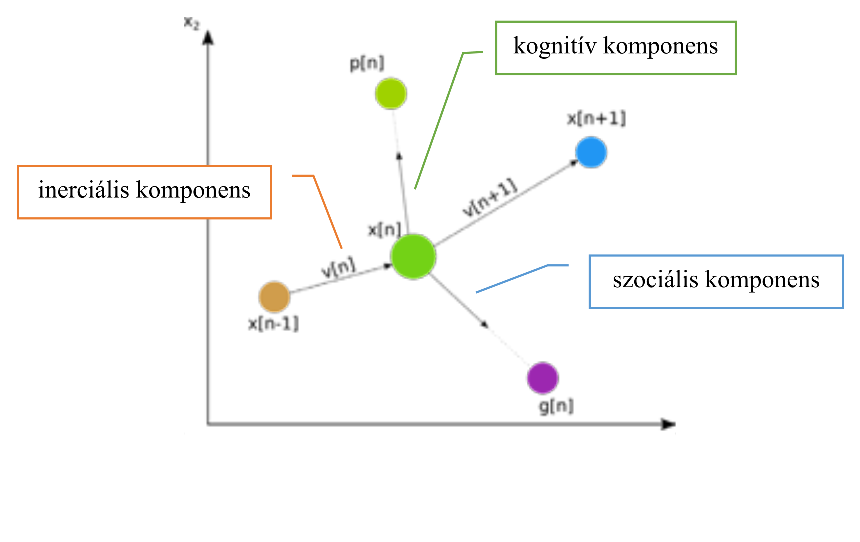
\includegraphics[width=0.8\textwidth]{komponensek}
    \caption{A részecske-raj optimalizáció komponensei \parencite{kanovic2017}}
    \label{fig:komponensek}
\end{figure}

Az algoritmus komponenseinek a kölcsönhatásait a \ref{fig:komponensek} ábra vizualizálja. Az egyes komponensek súlyozott értékei ($w$, $cp$ és $cg$) tetszőlegesen választhatóak, ebből eredendően több változata létezik a részecske-raj algoritmusnak. A dolgozatban bemutatott változatban ezek az együtthatók időben változó értékek, melyeknek az értékei a \ref{tab:psokomp} táblázatban találhatóak meg.

\begin{table}
    \centering
    \begin{tabular}{|c|c|c|}
    \hline
    együttható & kezdő érték & végső érték \\ \hline
    \hline
    $w$ & 0.9 & 0.4 \\ \hline
    $cp$ & 2.5 & 0.5 \\ \hline
    $cg$ & 0.5 & 2.5 \\ \hline
    \end{tabular}
    \caption{Az időben változó együtthatók értéke \parencite{kanovic2017}}
    \label{tab:psokomp}
\end{table}

\section{A részecske-raj algoritmus}

Első lépésként a raj nagyságát kell meghatározni, ami becslések alapján nagyjából tízszerese kell, hogy legyen a probléma dimenziójától \parencite{rapaic2019}. Erre azért van szükség, mert túl kevés egyed képtelen bejárni az egész keresési mező összes dimenzióját és információ hiányában nem kerül felderítésre lehetséges megoldások.

Az algoritmus elején minden részecskéhez véletlenszerűen egy kezdő pozíciót kell rendelni ($x[0]$), ami egyben az egyedek eddigi legjobb pozícióját is jelenti ($p[0]$). A kritériumfüggvény alapján kiszámoljuk melyik pozíció a legjobb, ez lesz a globális legjobb pozíció ($g[0]$). Ezzel lezárult az inicializációs rész.

A fő részben minden részecskének ki kell számolni a következő sebességét -- \ref{eq:vn} képlet, és ez alapján a pozícióját -- \ref{eq:xn} képlet. A részecske eddigi legjobb helyzetét is meg kell változtatni, ha az újabb pozícióra jobb eredmény születik. Miután bejeződött a ciklus, a globális pozíciót kell frissíteni úgy, hogy a részecskék eddigi legjobb pozícióinak az értékét hasonlítjuk össze a globálisan legjobb értékkel.

\linespread{1}
\begin{lstlisting}[caption={A részecske-raj algoritmus pszeudokódja \parencite{dorigo2008}}, captionpos=b]
begin pso-algoritmus
   %(*raj inicializáció*)
   while (%(*leállási feltétel nem teljesített*))
   do
      for (i=1 to %(*részecskék száma*))
         %(*sebesség és az új pozíció kiszámolása*)
         %(*kritériumfüggvény értékének meghatározása*)
         %(*részecske eddigi legjobb pozíciójának a frissítése*)
      end
      %(*globálisan legjobb pozíció frissítése*)
   end do
end pso-algoritmus
\end{lstlisting}

Leállási feltételként leggyakrabban egy előre megadott maximális ciklusszámot használnak, de ez függ a probléma típusától. Egy másik megoldás lehet a globálisan legjobb pozícióra kapott érték változását követni, miszerint ha egy megadott tűréshatár alá esik az érték változása, akkor teljesül a leállási feltétel \parencite{kanovic2017}.

\section{A részecske-raj algoritmus kivizsgálása}

A genetikus algoritmushoz hasonlóan, a részecske-raj algoritmus is demonstratív módon a Rastrigin-féle tesztfüggvény \ref{eq:rastrigin} által kerül elemzésre.

A fent leírt algoritmus alapján és a megfelelő paraméterek segítségével egy sajátkezűleg írt programot készítettem \textit{Python} programnyelvben \parencite{kisspy2020}. A vektorszámításokat a \textit{NumPy} könyvtár segítségével oldottam meg, míg az eredmények grafikonon történő megjelenítéséhez a \textit{matplotlib} könyvtárat használtam. A dolgozatban szereplő Rastrigin-függvény és minden egyéb grafikonos ábra szintén ezzel a szoftverrel készült el.

Az algoritmus elemzése négyféle környezetben zajlott, és mindegyik kísérlet 100-szoros ismétléssel történt. Az eredmények a \ref{tab:psores} táblázatban találhatók meg.

\begin{table}
    \centering
    \begin{tabular}{|c|c|c|c||c|c|c|}
    \hline
    \# & \rotatebox{90}{populációszám} & \rotatebox{90}{ciklusszám} & elhelyezés & átlageredmény & medián & szórás \\ \hline
    \hline
    \textbf{K1} & 25 & 100 & uniform & $0.3283$ & $8.7512 \cdot 10^{-12}$ & $0.4678$ \\ \hline
    \textbf{K2} & 25 & 1000 & uniform & $0.1194$ & $0$ & $0.3233$ \\ \hline
    \textbf{K3} & 25 & 100 & nem-uniform & $0.7960$ & $0.9950$ & $0.9850$ \\ \hline
    \textbf{K4} & 40 & 100 & nem-uniform & $0.3781$ & $1.5721 \cdot 10^{-13})$ & $0.6098$ \\ \hline
    \end{tabular}
    \caption{A részecske-raj optimalizáció elemzésének az eredményei}
    \label{tab:psores}
\end{table}

Az eredményekből egyértelműen látható, hogy az egyenletesen elhelyezkedő populáció esetében a ciklusszám növelése 100-ról 1000-re nem hatott ki az eredmény pontosságára, míg a nem egyenletesen elhelyezkedő populáció esetében a populáció számának a növelése nagyban javított az eredményen. Ez annak köszönhető, hogy az algoritmus komponenseinek az együtthatói időben változnak, így az idő múlásával csökken az egyedek felderítési hajlama, míg a szociális komponens erősödik. Ez azzal jár, hogy a kísérlet végére az egyedek egyre jobban hagyatkoznak az eddigi globálisan elért legjobb eredményre; így ha nem járták be a keresési mezőt, nagy valószínűséggel a legjobb eredmény egy lokális minimumban akad meg. A populáció számának a növelése esélyt ad a keresési mező jobb felderítésére, így megtalálva az optimális értéket.

Az algoritmus vizualizációja érdekében készítettem egy \textit{Javascript} programot, amely bármilyen böngészőből lefuttatható \parencite{kissjs2020}. A Rastrigin-féle függvény mellett még egyéb más tesztfüggvények is elérhetőek, melyekre (a kiválasztott paraméterek mellett) ki lehet számolni az optimális értéket (\ref{fig:psojs1} ábra). A számolás befejeztével megjelenik egy időcsúszkával ellátott grafikon (\ref{fig:psojs2} ábra), ahol végig lehet követni a populáció helyzetét a generációk folyamán. A raj animált mozgásának köszönve szemügyre vehető egy-egy részecske vándorlása valamint az egész populáció szintjén történő együttműködés, viselkedésminta.

\begin{figure}
    \centering
    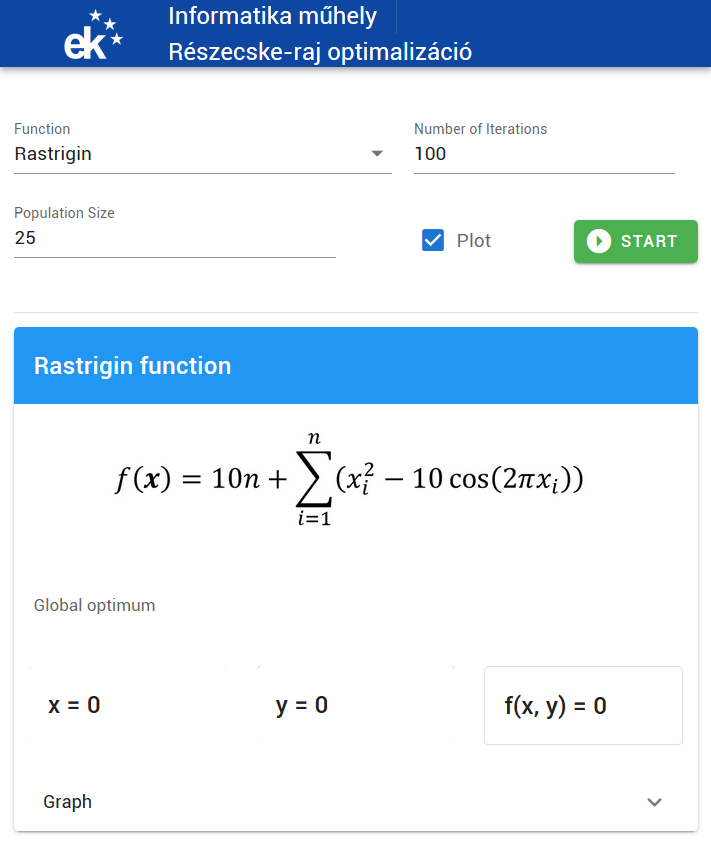
\includegraphics[width=0.6\textwidth]{psojs1}
    \caption{Paraméterek beállítása}
    \label{fig:psojs1}
\end{figure}

\begin{figure}
    \centering
    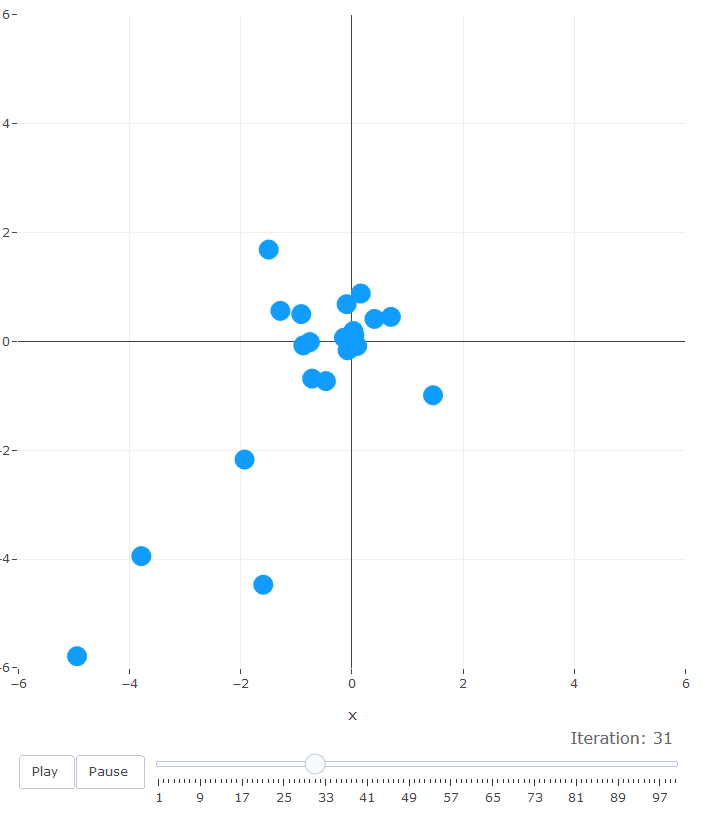
\includegraphics[width=0.6\textwidth]{psojs2}
    \caption{A részecskék időbeli mozgása}
    \label{fig:psojs2}
\end{figure}

\section{A részecske-raj algoritmus felhasználási területei}

Az algoritmus egyszerűségéből fakadóan sok szakterületen megállta a helyét, így pl. az egészségügyben leukémia-típusú problémák diagnózisában. Közgazdasági területen a kockázati befektetések elemzésére használják. Jelentkezik mechanikában, termodinamikában, valamint egyéb geometriai optimalizációs problémáknál is (pl. szenzorok optimális elhelyezése). Az optimális vezérlés, rendszermodellezés, károk észlelése és még sok más gyakorlati problémához kínál megoldást a részecske-raj algoritmus \parencite{almeida2019}.

A gyakorlati problémák mellett elméleti és más absztrakt témához is segítséget nyújt. A mesterséges intelligencia és a gépi tanulás kiképzési folyamatában valamint a mesterséges neuronhálózat paramétereinek optimális értékének a megkeresésében is használják a részecske-raj algoritmust \parencite{kanovic2017}.

\chapter{Következtetés}

A numerikus megoldásokkal szemben az evolúciós algoritmusok egyszerű és intuitív módon állnak hozzá az optimalizációs problémákhoz. Az egyedi problémák viszont egyedi megoldásokat is igényelnek; ilyenkor következetes módon kell kiválasztani a számunkra felkínált eszközöket, amik nem utolsó sorban a természet által inspirált optimalizációs megoldások is lehetnek.
Az elemzések során megfigyelhettük, hogy ezek az algoritmusok -- báris a kezdetleges változatuk -- nem minden esetben szolgált pontos eredménnyel. Manapság is aktív kutatási terület ezen algoritmusok további fejlesztése, ami még sok újdonságot hoz a mérnöki feladatok megoldásaiban.

\printbibliography[heading=bibintoc,title={Irodalomjegyzék}]

\printindex

\end{document}
